\documentclass{beamer}
\usepackage{scuwqt}
\usepackage{booktabs}
\usepackage{mathtools}
\usepackage{dzg-beamer}
\usepackage{tikzit}
\usepackage{dynkin-diagrams}
\usepackage{subcaption}
\setlength\parindent{2em}
\renewcommand{\arraystretch}{1.5}
%=========================================================
\title{Moduli of Coble Surfaces}
\author{D. Zack Garza}
\institute{NCTS}
\date{\today}
\setlength{\parindent}{2em}

\begin{document}
{

\begin{frame}
  \titlepage
\end{frame}
%=========================================================
{
    \usebackgroundtemplate{
        \tikz\node[at=(current page.west), yshift=-3cm]  {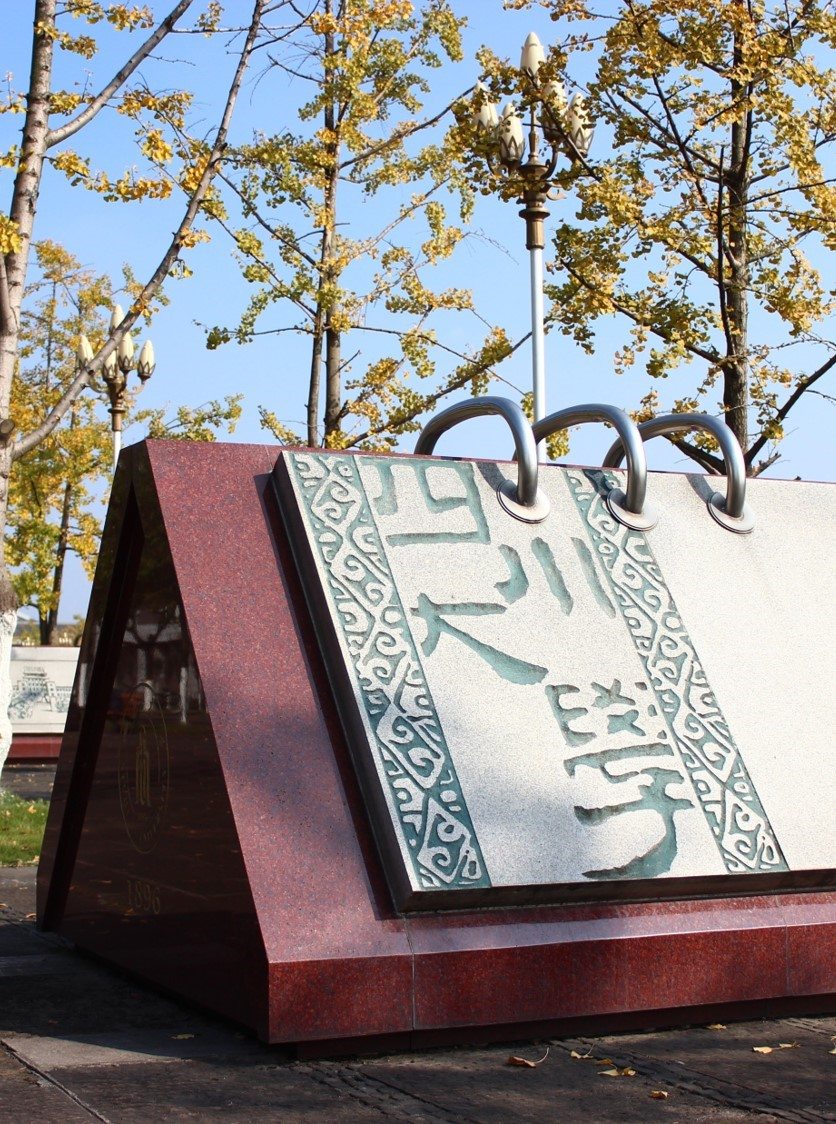
\includegraphics[width=0.5\paperwidth,height=\paperheight]{contents.jpg}};
    }

\begin{frame}

  \hfill 
  \begin{minipage}[t]{.4\textwidth} 
    \tableofcontents 
  \end{minipage}
\end{frame}}
%=========================================================

\section{Moduli of K3 Surfaces}

\begin{frame}
\frametitle{Introduction}
\begin{itemize}
\item K3 surface: \quad\hspace{0.6em} $q(X) \coloneqq h^1(\mathcal{O}_X) = 0$ and $\omega_X \cong \mathcal{O}_X$.
\item Enriques surface:  $q(X) = 0$ and $\omega_X \neq \mathcal{O}_X$ but $\omega_X^2 \cong \mathcal{O}_X$.
\item Coble surface: \hspace{1em} $q(X) = 0$, $h^0(\omega_X^{-1}) = 0$ but $h^0(\omega_X^{-2}) > 0$.
\end{itemize}
\vspace{1em}
\begin{centering}
{
\small
\begin{tabular}{l|llllll}
	Surface 	& $\mathrm{ord}(K_X)$ & $\kappa(X)$ 	& $\mathrm{Pic}(X)/\mathrm{tors}$ & $h^{2, 0}$ 
		& $h^{1,1}$ & $h^{0, 2}$ \\ \hline
	K3 			& $1$ & $0$ 			& $L_{K3} \coloneqq U^3 \oplus E_8^2$ 
		& $1$ & $20$ & $1$ \\
	Enriques 	& $2$ & $0$ 			& $L_{En} \coloneqq U \oplus E_8$ 
		& $0$ & $10$ & $0$ \\
	Coble 		& $\infty$ & $-\infty$ 		& $L_{Co} \coloneqq \gens{-1} \oplus U \oplus E_8$
		& $0$ & $11$ & $0$ \\
\end{tabular}
}
\end{centering}
\newline
{\small
\newline
Here $\gens{-1}$ is generated by $K_X$ where $K_X^2 = -1$.
}
\end{frame}
%=========================================================
\begin{frame}\frametitle{Lattices}
{
\[
\tiny 
G_U = \begin{pmatrix} 0 & 1 \\ 1 & 0 \end{pmatrix}, \qquad
G_{E_8}
=
\begin{pmatrix}
 -2 &  0 & 1 &  0 &  0 &  0 &  0 &  0 \\
 0 &  -2 &  0 & 1 &  0 &  0 &  0 &  0 \\
1 &  0 &  -2 & 1 &  0 &  0 &  0 &  0 \\
 0 & 1 & 1 &  -2 & 1 &  0 &  0 &  0 \\
 0 &  0 &  0 & 1 &  -2 & 1 &  0 &  0 \\
 0 &  0 &  0 &  0 & 1 &  -2 & 1 &  0 \\
 0 &  0 &  0 &  0 &  0 & 1 &  -2 & 1 \\
 0 &  0 &  0 &  0 &  0 &  0 & 1 &  -2
\end{pmatrix}.
\]
}

\[
\dynkin[edge length=1, root radius=0.1cm,labels={e, f}]{A}{xx}
\qquad
\dynkin[edge length=1, root radius=0.1cm, labels={\alpha_1,\alpha_2,\alpha_3,\alpha_4,\alpha_5,\alpha_6,\alpha_7,\alpha_8}]{E}{oooooooo},
\qquad
\]
\begin{align*}
\dynkin[edge length=0.5, root radius=0.1cm]{A}{x}: v^2 = 0, \qquad 
\dynkin[edge length=0.5, root radius=0.1cm]{A}{o}: v^2 = -2, \qquad
\dynkin[edge length=0.5, root radius=0.1cm]{A}{1}: v^2 = -4
\end{align*}
\end{frame}
%=========================================================
\begin{frame}
\frametitle{Nonsymplectic Involutions}


If $G\actson L$, define 
\[
L^G \da \ts{v\in L \st G.v = v} \leq L, \qquad L_G \da (L^G)^{\perp L}
\]

\begin{itemize}

\item $Y$ Enriques $\implies \exists X\to Y$ its universal cover by a K3.
\item $\pi_1(Y) = \gens{\iota_{\En}} \cong \ZZ/2\ZZ$ 
is a \textbf{nonsymplectic involution}: 
\[
\iota_{\En}(\sigma_X) = -\sigma_X \quad\text{where}\quad H^{2, 0}(X) = \CC\sigma_X
.\]

\item Yields 
\[
S_{\En} \coloneqq L_{K3}^{\gens{\iota_{\En}}} \cong L_{\En}(2) = U(2) \oplus E_8(2)
.\]

\item \cite{Nik79}: if $\iota\actson X$ is a nonsymplectic involution on a K3 surface, there are 75 possibilities for 
\[
S(\iota) \da \lkt^{\gens{\iota}}\quad\text{and}\quad T(\iota) \da S^{\perp \lkt}
.\]

\end{itemize}


\end{frame}
%=========================================================
\begin{frame}\frametitle{Nikulin's Pyramid}
\begin{center}
\begin{figure}[H]
\centering
\includegraphics[width=0.95\textwidth]{/home/dzack/.pandoc/figures/rendered/nikulin_lattice_pyramid}
\caption{$S_{\dP} = (2,2,0), S_{\En} = (10, 10, 0), S_{\Co} = (11, 11, 1)$.}
\end{figure}
\end{center}

\end{frame}
%=========================================================
\begin{frame}\frametitle{Period Domains}
For any lattice $T$ of signature $(2, n)$, there is a \textit{period domain} classifying Hodge structures of type $T$, a connected component of
\[
\Omega_T \da \ts{v\in \PP(T \otimes_\ZZ \CC) \st v^2 = 0, \bar{v}\cdot v > 0} = D_T \disjoint \overline{D}_T
.\]
Always a Type \IV Hermitian symmetric domain.
When $T$ is of geometric origin\footnote{e.g. $T = S^{\perp \lkt}$ for $S \injects \Pic(X)$ with $X$ a K3 surface.} and $\Gamma_T \leq \Orth(T)$ the monodromy group of the corresponding \textrm{ZVHS}, $\exists$ a moduli space $S$-polarized K3 surfaces
\[
F_T \da \dcosetl{\Gamma_T}{D_T}
.\]
\end{frame}
%=========================================================
\begin{frame}\frametitle{Existing Compactifications}
Examples:
{\tiny \begin{center}
\begin{tabular}{l|ll|ll|l}
	$\mcm$ & $S$ & $T$ & $S'$ & $T'$ & $\Gamma_T$ \\ \hline
	$F_{2d}$
		& $\gens{2d}$
		& $\gens{-2d} \oplus U^2 \oplus E_8^2$
		& $\I_{1,0}(2d)$
		& $\I_{0,1}(2d) \oplus \II_{2,18}$ 
		& $\Orth^+(T) \intersect \tilde{\Orth}(T)$ \\

	$F_{\mathrm{ell}}$\cite{ABE22}
		& $U$
		& $U^2 \oplus E_8^2$
		& $\II_{1,1}$
		& $\II_{2,18}$ 
		& $\Orth^+(T) \intersect \tilde{\Orth}(T)$ \\

	$F_{(2,2,0)}$\cite{AE22}
		& $U(2)$
		& $U \oplus U(2) \oplus E_8^2$
		& $\II_{1,1}(2)$
		& $\II_{1,1}(2) \oplus \II_{1,17}$ 
		& $\Orth^+(T) \intersect \tilde{\Orth}(T)$ \\

	$F_{\En}$\cite{Ste95a}
		& $U(2) \oplus E_8(2)$
		& $U \oplus U(2) \oplus E_8(2)$
		& $\II_{1,9}(2)$
		& $\II_{1,1} \oplus \II_{1,9}(2)$ 
		& $\Orth^+(T) \intersect \tilde{\Orth}(T)$ \\
		
	$F_{\En, h}$\cite{Ste95a}
		& $\cdots$
		& $\cdots$
		& $\cdots$
		& $\cdots$
		& $\Orth^+(T) \intersect \Gamma_{T, h}$ \\
\end{tabular}
\end{center}
}

Where
\[
\rho_T: \Orth(T) \to \Orth(A_T), \qquad h \da e + f \in S_{\En} = U(2) \oplus E_8(2)
,\]
\[
\Gamma_{T, h} = \rho_T\inv\qty{ \rho_S(\Stab_{\Orth(S)}(h) ) },
\qquad
\tilde{\Orth}(T) \da  \rho_T\inv(0)
.\]

{\tiny
(N.B.: $F_{2d}$ due to \cite{Sca87, Laz16, AET23}.)
}
% Why $O^+$: $O(T) \actson \Omega_T = D_T \disjoint \bar{D_T}$ does not fix $D_T$

\end{frame}
\section{Compactifications}
%=========================================================
\begin{frame}\frametitle{Compactifications}
By \cite{BB66}, $F_T$ is a quasiprojective variety.
When $\mcm$ is a moduli problem with coarse space $F_T$, there are many compactifications:
\[
\gitcpt{\mcm}, \quad
\bbcpt{F_T}, \quad 
\torcpt{F_T}, \quad
\semitorcpt{F_T}, \quad
\ksbacpt{\mcm}
.\]
For the KSBA compactifications, take pairs $(X, \eps R)$ where

{\small
\begin{tabular}{l|ll}
	$F_{2d}$ 
		& $(X, L), L^2=2d$
		& $R^{\rc} = \qty{ \displaystyle\sum_{\PP^1\cong C \in \abs{L}} n_C C}\in \abs{n_d L}$ 
		\\
	$F_{\mathrm{ell}}$ 
		& $(X, s + (d+1)f)$ 
		& $R^{\Ram} \da \Ram(X \mapsvia{2-\text{to}-1} \PP(1,1,4))$ 
		\\
	$\cdots$ 
		& $\cdots$ 
		& $R^{\rc} \approx s + \sum_{i=1}^{24} f_i$
		\\
	$F_{(2,2,0)}$ 
		& $(X, L)$ 
		& $R^{\Ram} \da \Ram(\iota_{\dP} \actson X)$ with $S = U(2)$
		\\
	$F_{\En, 2}$
		& $(Z, [L_Z])$ 
		& $R^{\Ram} \da \Ram(Z \mapsvia{2-\text{to}-1} \dP_4)$
		\\
\end{tabular}
}

\end{frame}
%=========================================================
\begin{frame}
\begin{theorem}[{\cite[Thm. 9.10]{AE22}}]
In 50 out of 75 cases for $T$, one has
\[
\semifancpt{F_T}{\mcf_\bullet(\Phi_{2, 4})} \to
\semifancpt{F_T}{\mcf_\bullet(\Phi_2)} \to
\semifancpt{F_T}{\mcf_\bullet^{\ram}}
\overset{\sim}{\longleftarrow}
\normalize{\qty{ \ksbacpt{F_T}}} 
\]
where $\mcf_\bullet^{\ram}$ is a collection of semifans indexed by $\bd_0 \bbcpt{F_T}$.
\end{theorem}
\vspace{2em}
{\small
\begin{align*}
\Phi(L) = \ts{\alpha \in L \st s_\alpha \in \Orth(L)}, 
\quad
\Phi_{2, 4}(L) \da \ts{\alpha \in \Phi(L) \st \alpha^2 = -2, -4}
\end{align*}
\[
s_\alpha(v) = v - (2v\alpha) \hat{\alpha}, \qquad \hat{\alpha} \da \alpha/\alpha^2
\]
}
\end{frame}
%=========================================================
\begin{frame}\frametitle{Stratified Spaces and Posets}
\ctikzsvg[width=0.83\linewidth]{tikz/compactification_posets_over_BB.tex}
\end{frame}

\section{Coble Surfaces}

%=========================================================
\begin{frame}\frametitle{Coble Surfaces}
\begin{definition}[Coble Surfaces]
A \textbf{Coble surface} \cite{Cob19, Oda85, DZ99, DM20} is a smooth, projective, rational surface $Y$ with 
\[
h^0(\omega_Y^{-1}) = 0, \,\, h^0(\omega_Y^{-2})\neq 0\qquad \qty{\iff \abs{-K_Y} = \emptyset,\,\, \abs{-2K_Y}\neq \emptyset }
.\] 
It is \textit{terminal of K3 type} if $\abs{-2K_Y} \ni C = \sum_{i=1}^n C_i$ with $C_i\cong \PP^1$ and $C_iC_j = -4\delta_{i=j}$. Write $F_{\Co} \da \ts{\text{Coble surfaces } Y}\modiso$.
\end{definition}
\begin{fact}
Every Coble is a basic rational surface: $\rho: Y\to \PP^2$ decomposes as a sequence of blowups at $N = 9+n$ points, and 
\[
\rho(C) \in \abs{-2K_{\PP^2}} = \abs{ \OO_{\PP^2}(6)}
.\]
\end{fact}
\end{frame}
%=========================================================
\begin{frame}\frametitle{Why Cobles are of interest}
In \cite{AEGS23} we construct $\cpt{ \fent} \cong \cpt{D_{\ten}/\Gamma_{\ten, 2}}$. By \cite{Nam85},
\begin{itemize}
\item \[ \ten[-2]/\Gamma_{\ten, 2} = \ts{\alpha}, \qquad \Delta_{-2} = \alpha^\perp \] are Coble surfaces with a ${(1,1)\over 4}$ singularity,
\item \[ \ten[-4]/\Gamma_{\ten, 2} = \ts{\beta_1, \beta_2}, \qquad \Delta_{-4} = \beta_1^\perp \union \beta_2^\perp, \]
\item $\beta_1^\perp$ are \textit{nodal} Enriques surfaces (resolution contains a $(-2)$-curve),
\item $\beta_2^{\perp}$ are \textit{unigonal} Enriques surfaces $Z \mapsvia{2-\text{to}-1} \PP(1,1,2)$.
\end{itemize}
{\small 
So $F_{\Co} \injects \fent$ as a divisor, as do $F_{\Nod}$ and $F_{\mathrm{uni}}$. So there exist KSBA compactifications of all three divisors.
}
\end{frame}
%=========================================================
\begin{frame}\frametitle{Coble Surfaces}
We primarily consider the $n=1$ case, so $K_Y^2 = -1$ and there are $N=10$ blowups.
\begin{construction}
Let $C \subseteq \PP^2$ be an irreducible rational sextic, then
\[
p_a(C) = { (d-1)(d-2)\over 2 } + \sum_{p\in C^\sing} \delta_p \implies \sum_p \delta_p = 10
.\]
\end{construction}
Choose $C$ with at worst slc singularities, then $C \in S_{6, 0}$ generically satisfies $C^\sing = A_1^{10}$ but admits many singularity profiles:
{\small
\begin{align*}
\delta(A_k) = \ceil[\big]{k/2} \leadsto & A_{20}, A_1^{10}, A_1^9 + A_2, A_1^8 + A_3, A_7 + A_6,  \\
&\quad  D_4 + A_1^7, E_6 + A_1^7, E_8 + A_1^6, \cdots
\end{align*}
}
\end{frame}
%=========================================================
\begin{frame}\frametitle{Coble Surfaces}
Then take $\rho: Y \da \Bl_{C^\sing}(\PP^2) \to \PP^2$, and $\tilde C \in\abs{-2K_Y}$ defines a 2-to-1 cover $\pi: X\to Y$ by a K3 surface $X$. We have
\[
\Pic(Y) = \Pic(\PP^2) \oplus \gens{E_1, \cdots, E_{10}} \cong \I_{1, 10}, \quad 
\pi^*: \Pic(Y)(2) \injects \lkt
\]
The image is a 2-elementary \cite{Nik79a} lattice, thus
\begin{align*}
S_{\Co} &\da \Pic(Y)(2) \cong \I_{1, 10}(2) &&\cong \gens{-2} \oplus U(2) \oplus E_8(2) = (11,11,11)_1 \\
T_{\Co} &\da S_{\Co}^{\perp \lkt} \cong \I_{2, 9}(2) &&\cong \gens{2} \oplus U(2) \oplus E_8(2) = (11,11,11)_2
\end{align*}
\[
\implies \exists \iota_{\Co}\actson X \,\text{nonsymplectic,}\,
\lkt^{\gens{\iota_{\Co}}} \cong S_{\Co},\,\,  \lkt_{\gens{\iota_{\Co}}} \cong T_{\Co}
\]
\[
\implies F_{\Co} \injects \cpt{ F_{\I_{1, 10}(2)} } = \cpt{ F_{(11,11,1)} } \text{ and } F_{\Co} \injects \cpt{ \fent } \injects \cpt{F_{(2,2,0)}}
.\]
\end{frame}

%=========================================================
\begin{frame}\frametitle{Coble Surfaces}
Note $F_{\Co} \subseteq (\PP^2)^{10}/\PGL_3$, and \cite{Cob19} shows there are 3 discriminant conditions, so $\dim{F_{\Co}} = 12-3$ agrees with $\dim( F_{\I_{1, 10}(2)} ) = 11-2$ and this is an open subset.

\begin{goal}
In \cite{AEGS23}, we show $\normalize{ \cpt{\fent} } \cong \semitorcpt{\fent}$ for a specific semifan.
Since $F_{\Co} \injects \cpt{\fent}$, its closure defines a KSBA compactification $\overline{F_{\Co}}$, and one can hope to recover $\partial \cpt{ F_{\Co}}$ from its intersection with $\partial \cpt{\fent}$:
\end{goal}

\begin{conjecture}
There is an isomorphism $\normalize{\cpt{F _{\Co}}} \iso \semitorcpt{F_{\Co}}$ where the semifan $\mcf$ can be made explicit, and stable models of degenerations of Coble surfaces can be effectively computed, giving an effective and complete description of $\partial \cpt{F_{\Co}}$.
\end{conjecture}

\end{frame}
\section{Boundaries}
%=========================================================
\begin{frame}
\ctikzsvg{tikz/m2_stable_graph_poset.tex}
\end{frame}
%=========================================================
\begin{frame}\frametitle{Stratification posets from Coxeter diagrams}
\ctikzsvg[width=\linewidth]{tikz/large_subdiagram_poset.tex}
\end{frame}
%=========================================================

%=========================================================
\begin{frame}\frametitle{Strategy}
{\small
\begin{itemize}
\item Compute the polarization $L_{Y_0}$ on a Coble central fiber $Y_0$ of a degeneration $(\mcz, \mcl_{\mcz} )$ of Enriques surfaces in $\fent$.
\item $\exists !$ open immersions of period domains
\[ F_{\Co} \injects F_{\I_{1, 10}(2)} \injects \fent \injects F_{(2,2,0)} \]
\item Compute the monodromy group $\Gamma_{\Co}$ and descend to quotients.
\item Construct $\bbcpt{F_{\Co}}$ and compute $\bd \bbcpt{F_{\Co}}$.
\item Compute the semifan refinement inducing $\semitorcpt{F_{Co}} \to \bbcpt{F_{\Co}}$ that coincides with $\cpt{F_{\Co}}$.
\item Compute the induced divisors $R_Y$ for induced stable pairs $(Y, \eps R_Y)$ in the closure of $F_{\Co}$ in $\cpt{\fent}$ or $\cpt{\fttz}$.
\item Compute the intersection of $\bd \cpt{F_{\Co}}$ with $\bd \cpt{\fent}$ lattice-theoretically.
\end{itemize}
}
%Cusp diagram: $\ftd, \fell, \fttz, \fent$
\end{frame}

%=========================================================
\begin{frame}\frametitle{Strategy}
{\small
\begin{itemize}
\item Use the fibration $\cpt{F_{\Co}} \to \bbcpt{F_{\Co}}$ to enumerate strata of $\bd \cpt{F_{\Co}}$.
\item Construct stable models as slices/restrictions/etc of stable models for $\bd \cpt{\fent}$, contracted from \textbf{integral affine} manifolds: $\PP^1(\RR)$ or $\DD$ folded from $\IAS^2$ for K3 surfaces.
\end{itemize}
}
\end{frame}
%=========================================================
\section{Work In-Progress}
\begin{frame}\frametitle{Preliminary Results}
\begin{theorem}
There are isometries
\begin{align*}
S_{\Co} &\cong \I_{1, 10}(2) \cong \gens{-2} \oplus U(2) \oplus E_8(2) = (11,11,1)_1 \\
T_{\Co} &\cong \I_{2, 9}(2) \cong \gens{2} \oplus U(2) \oplus E_8(2) = (11,11,1)_2
\end{align*}
\end{theorem}
\begin{theorem}
There is a primitive embedding of lattices
\begin{align*}
T_{\Co} \cong \gens{2} \oplus U(2) \oplus E_8(2) &\injects T_{\En} = U \oplus U(2) \oplus E_8(2) \\
h \oplus u \oplus \alpha &\mapsto (e+f) \oplus u \oplus \alpha
\end{align*}
\end{theorem}
\end{frame}
%=========================================================
\begin{frame}\frametitle{Prelimary Results}
{\small
\begin{theorem}
The sequence of primitive embeddings
\begin{align*}
T_{\Co} \injects T_{\En} \injects T_{(2,2,0)} \injects \lkt
\end{align*}
is unique (as a \textit{sequence} of embeddings) up to $\Orth(\lkt)$, and thus the corresponding maps on period domains are well-defined.
\end{theorem}
\begin{theorem}
The quotient $F_{\Co} \da D_{T_\Co} / \Orth^+(T_\Co)$ is a moduli space of \textbf{unpolarized} Coble surfaces, and there is a moduli space $F_{\Co, 2} \da D_{T_{\Co}}/\Gamma_{T_{\Co}, 2}$ of \textbf{polarized} Cobles surfaces.
If the unique orbit $\delta$ in $T_{\En}[2]/\Orth^+(\ten)$ remains unique in $T_{\En}[2]/\Gamma_{\En, 2}$, then there are identifications
\[
\Gamma_{T_{\Co}, 2} \cong \im( Z_{\Orth(\ten)} (\delta) \to \Orth(\delta^\perp) ) \text{ and } \delta^\perp \cong T_{\Co}
.\]
\end{theorem}
}

\end{frame}
%=========================================================
\begin{frame}\frametitle{Coble Surfaces}
\begin{theorem}\label{thm:cusp_correspondence}
The morphism $\eta: F_\Co\to F_\En$ (unpolarized!) extends to an morphism $\bd \bbcpt{F_{\Co}} \to \bd \bbcpt{F_{\En}}$:

\ctikzsvg[width=0.6\linewidth]{tikz/fig_Cusp_Correspondence_Co_En.tex}

\end{theorem}
{\tiny
Why: by \cite{KK72}, this is because (1) both sides are \textit{bounded} symmetric domains, (2) $\eta$ is holomorphic, (3) both groups are arithmetic, (4) $\eta$ is equivariant, and (5) HSDs are hyperbolically embedded in their Baily-Borel compactifications.
}
\end{frame}
%=========================================================
\begin{frame}\frametitle{Coble Surfaces}
{\small
\begin{conjecture}[Pending computation!]
$\bd\bbcpt{F_{\Co, 2}}$ has four 0-cusps and maps to $\bd\bbcpt{\fent}$ as follows:
\ctikzsvg[width=0.7\linewidth]{tikz/coble_to_sterk_f_en_2_cusp_diagram.tex}
\end{conjecture}
\tiny
Idea: choose $\delta = e-f$, show $v_i \perp \delta$ for $i=2,3,4,5$ \cite{Ste91} and $v_1\not\in\delta^{\perp} = T_{\Co}$: $T_{\Co}$ is even and $\div_{T_\En}(v_1) = 1$.
Check that $\bar{v_i} \in A_{T_{\Co}}$ yield distinct $\bar{\Orth^+(T_\Co)}$ orbits, lift, argue non-splitting under $\Gamma_{\Co, 2}$.
}
\end{frame}
%=========================================================
\begin{frame}\frametitle{Coble Surfaces}
\begin{theorem}
$F_{\Co, 2}$ is the normalization of a closed subvariety of $F_{\En, 2}$.
\end{theorem}
{\small
Idea: restrict $T_{\Co}/\Gamma_{\Co, 2} \to T_{\En}/\Gamma_{\En, 2}$ to scheme theoretic image $\implies$ birational. Proper and quasi-finite (because finite index subgroup) $\implies$ finite. Both are normal by \cite{BB66}; apply Zariski's main theorem and identify image with a Noether-Lefschetz locus.
}
\begin{conjecture}
{\small
Let $X\to \tilde Y$ be the K3 cover of a Coble surface, with $Y = X/\iota_{\iota_{\Co}}$. Then $\iota_{\Co}$ is the limit of an Enriques involution $\ien$ which commutes with a \textit{del Pezzo involution} $\idp\actson X$. Thus $\idp\actson Y$ yields an ample $\QQ$-Cartier ramification divisor. Resolving the $\frac{ (1,1)}{ 4}$ singularity $Y\to \tilde Y$, the pair \[ (Y, \frac{1 + \eps}{2} C + \eps \Ram(\idp)) \] 
is KSBA stable and induced by taking the closures $F_{\Co} \injects \cpt{\fent} \injects \cpt{\fttz}$.
}
\end{conjecture}
\end{frame}

\begin{frame}
\begin{theorem}
For the unique $v_0 \in T_{\Co}[0]/\Orth^+(T_\Co)$, there is an identification
\[
v_0^\perp / v_0 \cong \gens{2} + E_8(2) \cong (9,9,1)_1
\]
whose Coxeter diagram is obtained from $\fent$ by restriction:

\ctikzsvg{tikz/k3-to-enriques-to-coble.tex}
\end{theorem}
\end{frame}

\begin{frame}
\begin{center}
\includegraphics[width=0.7\linewidth]{screenshots/f-en-2-folding.png} 
\includegraphics[width=0.5\linewidth]{screenshots/example-ias2.png}
\end{center}
\end{frame}

%%%%%%%%%%%%%%%%%%%%%
\begin{frame}\frametitle{$\IAS^2$ and dlt models}
\begin{center}
\includegraphics[width=\linewidth]{screenshots/f-en-2-stable-models}
\end{center}
{\tiny
Surfaces appearing as (double covers of) irreducible components in divisorial log terminal models:
\begin{itemize}
\item $\Bl_{4\tor}(\PP^1\times \PP^1)$
\item $\Bl_{2\tor}\FF_4$
\item $\Bl_{2\mathrm{Nontor}}(\PP^1\times \PP^1)$
\item $\FF_2$
\item An $A_{15}$ $\ADE$ surface
\end{itemize}
One takes the corresponding integral affine manifolds and performs contractions to obtain KSBA stable models.
}
\end{frame}

\begin{frame}\frametitle{Irreducible components of KSBA Stable Models}

\begin{figure}
\centering
\begin{subfigure}{.30\textwidth}
  \centering
  \ctikzsvg[width=\linewidth]{tikz/ade-surface-diagrams/A3.tex}
\end{subfigure}
\hfill
\begin{subfigure}{.30\textwidth}
  \centering
  \ctikzsvg[width=\linewidth]{tikz/ade-surface-diagrams/minus-A3.tex}
\end{subfigure}
\hfill
\begin{subfigure}{.30\textwidth}
  \centering
  \ctikzsvg[width=\linewidth]{tikz/ade-surface-diagrams/A4-minus.tex}
\end{subfigure}

\vspace{1em}

\begin{subfigure}{.30\textwidth}
  \centering
  \ctikzsvg[width=\linewidth]{tikz/ade-surface-diagrams/D4.tex}
\end{subfigure}
\hfill
\begin{subfigure}{.30\textwidth}
  \centering
  \ctikzsvg[width=\linewidth]{tikz/ade-surface-diagrams/E6.tex}
\end{subfigure}
\hfill
\begin{subfigure}{.30\textwidth}
  \centering
  \ctikzsvg[width=\linewidth]{tikz/ade-surface-diagrams/E8-tilde.tex}
\end{subfigure}
\end{figure}

\end{frame}

\begin{frame}[allowframebreaks]{References}

\bibliographystyle{alpha}
{\tiny
\bibliography{/home/dzack/.pandoc/bib/references}
}
\end{frame}


\end{document}